  This is the technical core of the thesis. Here you lay out your how
  you answered your research question, you specify your design of
  experiments or simulations, point out difficulties that you
  encountered, etc.

  (target size: 3-4 pages)
  
  \subsection{Data Description and Preprocessing}
  
  \indent \indent
  		The data set used for this experiment was obtained from Kaggle (a platform for predictive modelling and analytics competitions). The data set was provided by Google for a web traffic prediction competition.
		 This data file consists of  number of views for 145063 Wikipedia pages on each date starting from 1$^{st}$ of July 2015 to 31$^{st}$ of December 2016. Each time series consists of data for the traffic generated by humans or bots or both from devices like mobile or desktop .
		 For each date, the data contains a single integer value representing the number of views that a particular Wikipedia page received on that date.  The total length of each time series is 550. There are some missing values for some of the time series. In this experiment, we have ignored such time series for the sake of convenience. Out of 145063 time series, we have chosen the traffic generated for page named "2002 FIFA World Cup" on english version of Wikipedia i.e \url{https://en.wikipedia.org/} on desktop devices by all types of agents including humans and bots. \\
		 		% Some of the raw time series data chosen for this experiment are visualized in Figure \ref{fig:raw}\subref{fig:raw_12} and Figure \ref{fig:raw}\subref{fig:raw_15}.
		 
		\begin{figure}
		     \centering
		     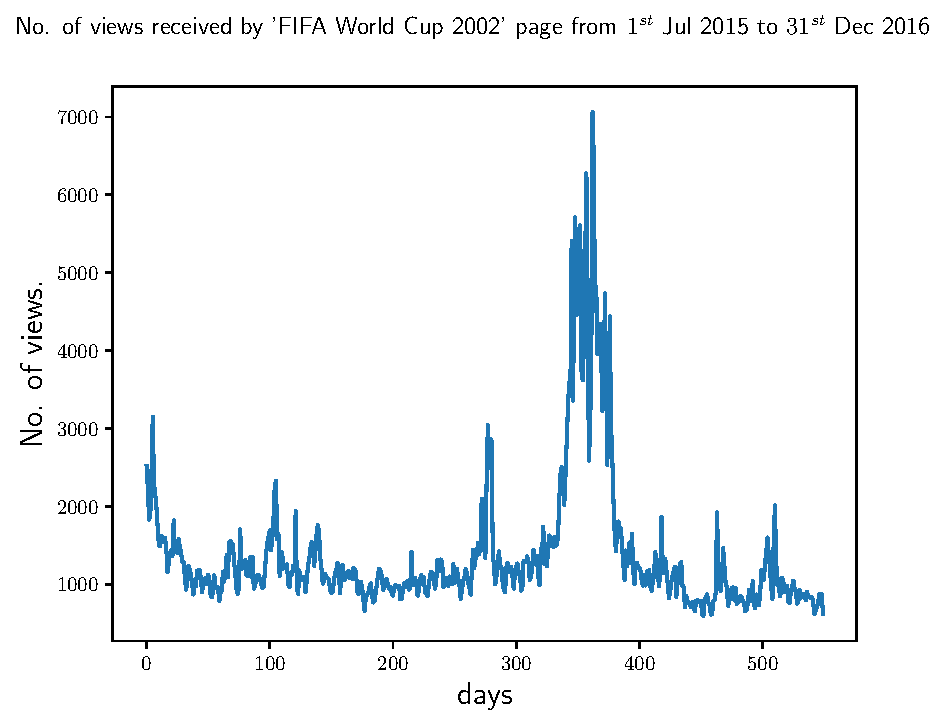
\includegraphics[width = 15cm]{./description/images/rawSignal}
			   
			   \caption{Raw data which has number of views of Wikipedia Pages on each date from 1$^{st}$ of July  2015 to 31$^{st}$ of December 2016. }
			\label{fig:raw}
			\end{figure}
			
For the preprocessing of the time-series following steps are followed:
\subsubsection{Step 1}
The time series data used in this experiment has very large values ($\approx  7000$) as seen in the the Figure \ref{fig:raw}.  Therefore, the time-series data is squeezed component wise such that the maximum value, $MAX$ of the time-series is squeezed to the new maximum value $max$. This is done by taking small ($< < 1$) power of each component in time series $\mathbf{s}(n) = (s(1),\hdots,s(n))$. The power $p$ that need to be raised to each component of time-series is calculated using Eq. \ref{eq:power}.  

\begin{equation}
\begin{split}
		max &= MAX^p\\
		p &= log_{MAX}(max)
\end{split}
\label{eq:power}
\end{equation}

\subsubsection{Step 2}
   The resultant time series from step 1 is further rescaled and shifted such that it has zero mean and unit variance. The time-series data is divided component wise by its standard deviation to make its variance unit. 
   
\subsubsection{Step 3}
  The resultant time series from step 2 is further applied a $tanh$ function component wise. This strictly scales the data points in time series in the range of $-1$ to $1$.
  
  \begin{figure}[h]
      % \centering
      \begin{subfigure}[h]{0.5\textwidth}
          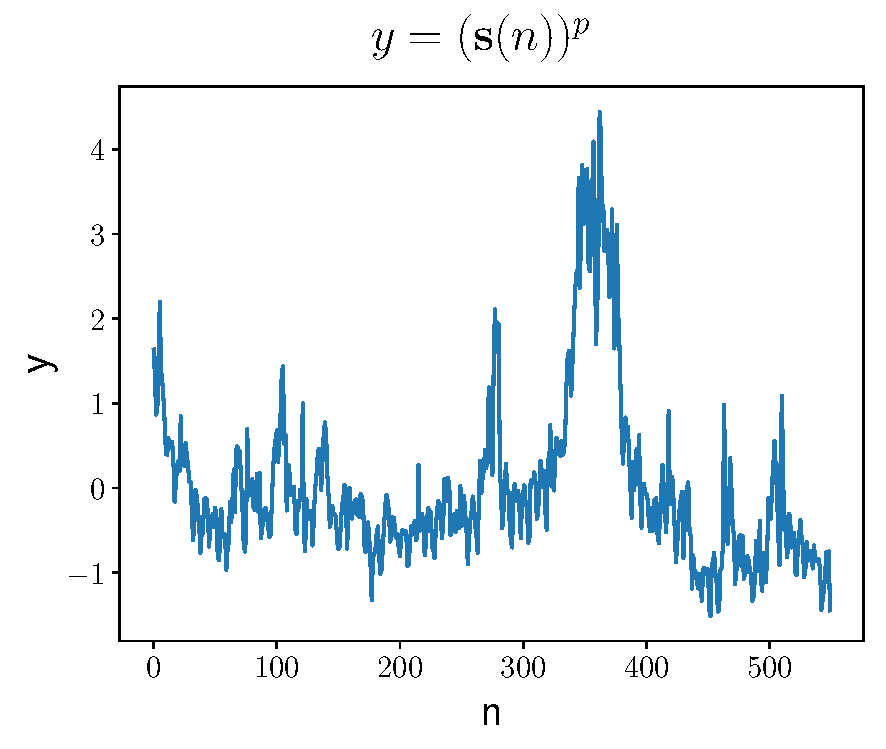
\includegraphics[width=\textwidth]{./description/images/squeezed}
          \caption{ After taking component-wise power}
          \label{fig:squeezed}
      \end{subfigure}
       %add desired spacing between images, e. g. ~, \quad, \qquad, \hfill etc. 
        %(or a blank line to force the subfigure onto a new line)
      \begin{subfigure}[h]{0.5\textwidth}
          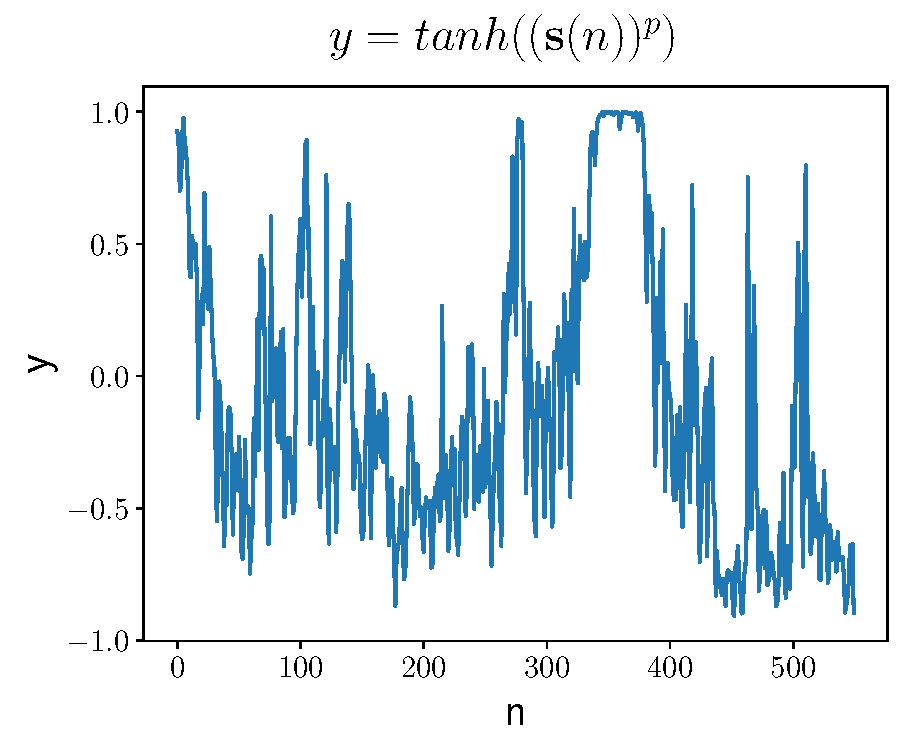
\includegraphics[width=\textwidth]{./description/images/tanh}
          \caption{After further taking the $tanh$ of the signal}
          \label{fig:tanh}
      \end{subfigure}
     
      \caption{Preprocessing steps}\label{fig:animals}
  \end{figure}
  
 \subsection{Additional Input Signals}

 
 \indent \indent
 By nature, the number of views that a particular Wikipedia Page receives vary according to  days in week and months in a year. For instance: A page related to weekend activities might receive a different proportion of views on weekends than on working days. Further, Wikipedia pages that on related subject matters might receives proportional number of views and could follow similar pattern of incoming web traffic. Therefore those related input signals were added to the ESN to improvise the prediction result. In particular we used following approach to find suitable additional input for the network. \\\\
 
 \begin{enumerate}
	 \item First of all a sine wave of period 7 was searched which has highest correlation with the main input signal. 
	 \item Then from the data base of about 145 thousand time series top 20 time series are selected with has highest correlation with the main input signal. These signals are further preprocessed using the same preprocessing routines as used for preprocessing the main input signal. To determine the correlation between two time series we have used Pearson's correlation coefficient.
	 
 \end{enumerate}
 
 
 
 \subsubsection{Pearson correlation coefficient}
  Pearson's correlation coefficient is the measure of the linear correlation coefficient between two variables. It's value is in the range of -1 to 1. Value close to 1 indicate that the variables are highly correlated to each other and values close -1 indicates that the variables are negatively correlated to each other and values close to 0 indicates that the two variables are unrelated. Pearson coefficient between to time series $\mathbf{X} = (x_1, \hdots, x_m)$ and $\mathbf{Y} = (y_1, \hdots, y_m)$ can be computed using the Equation %\cite{eq:pearson}
  
  \begin{equation}
  \begin{split}
	  \rho X,Y =& \frac{cov(X,Y)}{\sigma_X \sigma_Y}\\
		=& \frac{\Sigma^{m}_{i=1}(x_i - \bar{x})(y_i - \bar{y})} {\sqrt{\Sigma^m_{i=1}(x_i - \bar{x}^2)}}
  \end{split}
   \label{eq:pearson}
  \end{equation}
  
  where:
  \begin{itemize}
	  \item $m$ is the length of time series
	  \item $x_i, y_i$ are the data points in time series $X$ and $Y$ indexed with $i$
	  \item $\bar{x_i} = \frac{1}{n}\Sigma_{i=1}^{n}x_i$  and analogously for $\bar{y}$
	  
	  \end{itemize}
 
 
 So to give the insight of weeks and months, two additional input signals with periods 7 and 30 $\pm$ 2 were introduced to the network. These periodic signals were preprocessed (applied log10 and shifted by its mean) before feeding it to the network.



		% Max &= \text{max}\left( \mathbf{s}(n)  \right) \\
	% 	Max^p = \text{max}\left( \mathbf{s}(n)  \right) ^p\\
	% 	max &= \text{max}( (s(1),\hdots,s(n)) 
% \end{multline}
	% \begin{multiline}
% 		max = \text{max}( \mathbf{s}(n)  ^p \\
% 		max = \text{max}( (s(1),\hdots,s(n)) ^p
% 	\end{multiline}
%


\subsection{Network Setup}
\indent \indent
    Under suitable conditions the network state becomes asymptotically independent of initial conditions and depends only on the input history, which is called the "Echo State Property". This means that all desired output signals can be build out of it's own "echos" in the Dynamic Reservoir. \cite{ESNinAudioProcessing}\\
	We create a reservoir of $N = 99$ neurons. %The weights of each synaptic links connecting the neurons of reservoirs are chosen randomly from uniform distribution over (-0.5, 0.5). These weights are stored in  weight matrix $\mathbf{W}\in \mathbb{R}^{N\times N}$.
	   The weights  for input links  
	 and bias vector 
	 are generated randomly from uniform distribution over (-0.5, 0.5) and stored in matrix $\mathbf{W}^{in} \in \mathbb{R}^{N\times K}$  and $\mathbf{B} \in \mathbb{R}^{N\times 1}$ respectively. Then 
	 $\mathbf{W}$ matrix is normalized by its maximum eigenvalue. There are $K=22$ input neurons that receive each of the $21$ input signals and $L=31$ output neurons each of which makes $t=1,\hdots,31$ step ahead prediction.
\\

In order to achive good approximation of desired signal, the echo functions should provide a "rich" set of dynamics to combine from. The network should be prepared in a suitably "inhomogeneous" way to meet this demand. One simple method to prepare such a "rich reservoir" echo state network is to supply a network which is sparsely and randomly connected. Sparse connectivity provides for a relative decoupling of subnetworks, which encourages the development of individual dynamics \cite{shortTermMemory}. In this experiment, the network weight matrix, $\mathbf{W}$ has different weight regions to create different capability of short term memory so that the network can capture all type of trend (slow, medium and fast trends) in the training signal. The structure of weights matrix used is presented below:\\
      \begin{center}
	  \begin{tabular}{|l|r|c|}\hline
		  \
		  fast & $\approx$ 0 & =0 \\[5ex] \hline
		  $\approx$ 0 & medium & $\approx$ 0 \\[5ex] \hline
		  =0 & $\approx$ 0 & slow \\[5ex] \hline 
	  \end{tabular}	  
	  \end{center}
The fast region of matrix $\mathbf{W}$ has values in range $0.7$ to $1.0$, medium region as values in range $0.4$ to  $0.7$ and the slow region has values in range $0.0$ to $0.3$ generated randomly from the uniform distribution.  The weight matrix $\mathbf{W}_0$ is normalized to  $\mathbf{W}_1$ with it's spectral radius  by putting $\mathbf{W}_1 = \left| 1/\lambda _{max}\right| \mathbf{W}_0$ where $\lambda _{max}$ is the spectral radius of $\mathbf{W}_0$. Then the weight matrix $\mathbf{W_1}$ is scaled with a scaling factor $sf_W$ such that $\mathbf{W} = sf_W \mathbf{W_1}$. Then $\mathbf{W}$ has spectral radius of $sf_W$. The choice of the spectral radius $sf_W$ of the reservoir is crucial for the eventual success of ESN training. This is because $sf_W$ is  intimately connected to the intrinsic timescale of the dynamics of the reservoir state. Small $sf_W$ means that one has a fast dynamics reservoir and large $sf_W$ (i.e close to unity) means that one has slow reservoir. Also the input weight matrix $\mathbf{W}^{in}$  and bias vector $\mathbf{B}$ is scaled with a scaling factors $sf_Win$ and $sf_B$ respectively. 

\subsection{Regularization}
In order to access the quality of the prediction produced by the training of ESN, we regularly monitor the actual obtained output weights $\mathbf{W}^{out}$. Large weights indicate that $\mathbf{W}^{out}$ exploits and amplifies tiny differences among the dimension of  $\mathbf{x}(n)$, and can be very sensitive to deviations from the exact conditions in with the network has been trained \cite{mantas}. To counteract this effect the regularization part $\beta \mathbf{I}$ in the ridge regression is used as in Equation  \eqref{eq:wout} .

\subsection{Leaking Rate}

The leaking rage $\alpha$ of the reservoir nodes can be regarded as the speed of the reservoir update dynamics discretized in time. 
